\documentclass[article, a5paper]{memoir}

\let\footruleskip\undefined\usepackage{fancyhdr}% http://ctan.org/pkg/fancyhdr

\usepackage{pgfpages}
\pgfpagesuselayout{resize to}[a4paper]

% Swedish.
\usepackage[utf8]{inputenc}
\usepackage[T1]{fontenc}
%\usepackage[swedish]{babel}
\usepackage{microtype}

%%% FONT PACKAGES
%\usepackage[sc]{mathpazo}
%\usepackage[varg]{txfonts}
%\usepackage{times}
%\usepackage{tgtermes}% clone of times
%\usepackage[sfdefault,condensed]{cabin}
\usepackage{PTSansNarrow}\renewcommand*\familydefault{\sfdefault}
%\usepackage{tgcursor}
\usepackage[scaled=0.85]{beramono} % inconsolata or beramono ???
%\usepackage{fouriernc} % serif: new century schoolbook
%\usepackage{avant}     % sans serif: Avant Garde


% Typeblock size, margins.
\settypeblocksize{190mm}{127mm}{*}
\setlrmargins{10.5mm}{*}{*}
\setulmargins{10.0mm}{*}{*}
\setheadfoot{0.1pt}{0.1pt}
\checkandfixthelayout
\usepackage{multicol} \setlength{\columnsep}{5mm}
\usepackage{xcolor}
\usepackage{array}

\definecolor{mygreen}{rgb}{0,0.4,0}
\definecolor{grammarcolor}{rgb}{0.3,0.6,0.1}
\definecolor{mylinkcolor}{rgb}{0,0.1,0.5}
\definecolor{myemphcolor}{rgb}{0,0.4,0.1}
\definecolor{myalertcolor}{rgb}{0.4,0.1,0}
\definecolor{eclipsepurple}{rgb}{0.5,0,0.25}
\definecolor{eclipseblue}{rgb}{0.16,0,1.0}
\definecolor{eclipsegreen}{rgb}{0,0.5,0}


\newcommand{\OptL}{\textbf{\textcolor{grammarcolor}{[}}}
\newcommand{\OptR}{\textbf{\textcolor{grammarcolor}{]}}}
\newcommand{\RepL}{\textbf{\textcolor{grammarcolor}{(}}}
\newcommand{\RepR}{\textbf{\textcolor{grammarcolor}{)}}}
\newcommand{\Or}{\textbf{\textcolor{grammarcolor}{|}}}

%---------------------------------------------------------------

\newcommand{\LangColor}{red}

\setlength{\parindent}{0pt}
\raggedright
\raggedbottom
\linespread{0.90}\selectfont
\pagestyle{empty}

\newcommand{\mc}[1]{\multicolumn{2}{l}{\hspace{-0.65em}\parbox[t]{102mm}{\small #1}}}

\newcommand{\ind}{\hspace*{1.5em}}

\newcommand{\head}[1]{{\bfseries {\color{\LangColor}{#1}}\par\vspace{1mm}\hrule\vspace{-2mm}}}

\newenvironment{etab}%
{\begin{ctabular}{@{}>{\raggedright\small}p{25mm} @{}>{\raggedright\small}p{45mm} @{}>{\raggedright\arraybackslash\small}p{57mm}}}
{\end{ctabular}}%


\newcommand{\secend}{\\[1mm]}
\newcommand{\subsecend}{\\ \\[-2mm]}
\renewcommand{\arraystretch}{0.9}

% -----------
\usepackage{tikz}
\usetikzlibrary{calc}
\usetikzlibrary{shapes.geometric, shapes.symbols, arrows, matrix, shapes, positioning}
%https://www.sharelatex.com/blog/2013/08/29/tikz-series-pt3.html
\tikzstyle{startstop} = [rectangle, rounded corners, minimum width=3cm, minimum height=1cm,text centered, draw=black, fill=red!30]
\tikzstyle{io} = [trapezium, trapezium left angle=70, trapezium right angle=110, minimum width=1cm, minimum height=1cm, text=white, text centered, draw=black, fill=blue!50!violet]
\tikzstyle{process} = [rectangle, minimum width=3cm, minimum height=1cm, text=white, text centered, draw=black, fill=red!50!black]
\tikzstyle{decision} = [diamond, minimum width=3cm, minimum height=1cm, text centered, draw=black, fill=green!30]
\tikzstyle{arrow} = [thick,->,>=stealth]
%UML definitions
\tikzstyle{umlclass}=[rectangle, draw=black,  thick, anchor=north, text width=3cm, rectangle split, rectangle split parts = 3]
\tikzstyle{umlarrow}=[->, >=open triangle 90, thick]

%%%%%%%%%%%%%%%%%%%%%%%%%%%%
%%% lingstings specifics:
\usepackage{listings}
\usepackage{upquote} %http://tex.stackexchange.com/questions/145416/how-to-have-straight-single-quotes-in-lstlistings
\lstdefinelanguage{Scala}{
  morekeywords={abstract,case,catch,class,def,%
    do,else,extends,false,final,finally,%
    for,forSome,if,implicit,import,lazy,match,%
    new,null,object,override,package,%
    private,protected,return,sealed,%
    super,this,throw,trait,true,try,%
    type,val,var,while,with,yield},
  otherkeywords={=>,<-,<\%,<:,>:,@},
  sensitive=true,
  morecomment=[l]{//},
  morecomment=[n]{/*}{*/},
  morestring=[b]",
  morestring=[b]',
  morestring=[b]"""
}


\lstset{
    language=Scala,
    tabsize=2,
    basicstyle=\ttfamily\selectfont,
    keywordstyle=\bfseries\textcolor{eclipsepurple},
    commentstyle=\textcolor{mygreen},
    numberstyle={\footnotesize},
    numbers=none,
    %backgroundcolor=\textcolor{gray!15},
    frame=none,
    rulecolor=\color{black!25},
    %title={\footnotesize\lstname},
    breaklines=false,
    breakatwhitespace=false,
    framextopmargin=2pt,
    framexbottommargin=2pt,
    showstringspaces=false,
    columns=fullflexible,keepspaces
}
\lstset{literate=%
{Å}{{\AA}}1
{Ä}{{\"A}}1
{Ö}{{\"O}}1
{Ü}{{\"U}}1
{ß}{{\ss}}1
{ü}{{\"u}}1
{å}{{\aa}}1
{ä}{{\"a}}1
{ö}{{\"o}}1
{æ}{{\ae}}1
{ø}{{\o}}1
{Æ}{{\AE}}1
{Ø}{{\O}}1
{`}{{\`{}}}1
{─}{{\textemdash}}1
{└}{{|}}1
{├}{{|}}1
{│}{{|}}1
}

\newcommand{\code}{\lstinline[basicstyle=\ttfamily]}
\newcommand{\jcode}{\lstinline[basicstyle=\ttfamily,language=Java]}

\lstnewenvironment{Code}[1][]{%
    \lstset{basicstyle=\ttfamily\fontsize{10}{12}\selectfont,#1}%
}{}

%*****************************************************************



\newcommand{\LangRect}[4]{\tikz[overlay, remember picture,inner sep=7pt,minimum height=0.65cm] \node[fill=#2,text=white,rotate=90] at #4 (name) {\large\normalfont\textbf{#1} ~~{\small \thepage(4)}}; }  

\newcommand{\LangRectOdd}[3]{\LangRect{#1}{#2}{#3}{($(current page.north east)-(0.35,#3)$)}}  
\newcommand{\LangRectEven}[3]{\LangRect{#1}{#2}{#3}{($(current page.north west)-(-0.35,#3)$)}}  
    

\newcommand{\LangMarker}[2]{%param 1 = language, param 2 = offset from top
%\fancyhead{} % clear all header fields
\fancyfoot{} % clear all footer fields
%\fancyfoot[RO]{\thepage}
%\fancyfoot[LE]{\thepage}
\fancyhead{
\ifodd\thepage\LangRectOdd{#1}{\LangColor}{#2}
\else\LangRectEven{#1}{\LangColor}{#2}
\fi
}
\renewcommand{\headrulewidth}{0pt}
\renewcommand{\footrulewidth}{0pt}
\pagestyle{fancy}
}

\newcommand{\Newline}{\vspace{\baselineskip}}

\newcommand{\LangTitle}[1]{{\centering \Huge{\bfseries\sffamily \color{\LangColor}{#1}}\par\Newline}}



\begin{document}

\LangMarker{Scala}{1.5cm}
\LangTitle{Scala Quick Reference}


\head{Expressions}\Newline

{\small\renewcommand{\arraystretch}{1.1}
\begin{tabular}{l l p{6.5cm}}
literals  &  \code|0 0L 0.0 "0" '0' true false|   & Basic types e.g. Int, Long, Double, String, Char, Boolean \\
block     &  \code|{ expr1; ...; exprN } |         &  The value of a block is the value of its last expression   \\
if        &  \code|if (cond) expr1 else expr2 |  &   The value is expr1 if cond is true else expr2 \\
for       &  \code|for (x <- xs) expr |          &   Loop for each x in xs, x visible in expr, type Unit   \\
yield     &  \code|for (x <- xs) yield expr|     &   Yeilds a sequence with elems of expr for each x in xs \\
while     &  \code|while (cond) expr |           &   Loop expr while cond is true, type Unit \\
do while  &  \code|do expr while (cond) |        &   Dp expr at least once and then while cond is true, type Unit \\
throw     &  \code|throw new Exception("Bang!") |  &  Throws an exception that halts execution if not in try catch  \\
try       &  \code|try expr catch pf |           & Evaluate partial function pf if exception in expr, where pf e.g.: 
\code|{case e: Exception => someBackupValue}| \\ 


\end{tabular}
}

{\small
\begin{tabular}{r l | r  p{5cm}}\hline\\
\textbf{Precedence} & in operator notaion & Example expressions:& Explanation, x, i, j are integers \\
\textbf{Lowest} & all letters  & \code|(x + 2) * i / 3| & Parenthesis control order of evaluation \\
 & \code+|+       &  \code|1.+(2)|      & Method application, call method + on object 1\\
 & \code|^|       &  \code|1 + 2|       & Operator notation equivalent to 1.+(2)\\
 & \code|&|       &  \code|x < y|       & Yields true or false, other ops: > <= >= == !=\\
 & \code|= !|     &  \code|cond1 && cond2|& Logical and, other boolean ops are or: || not: !\\
 & \code|< >|     &  \code|f(1, 2, 3)|  & Function application, same as f.apply(1,2,3)\\
 & \code|:|       &  \code|x => x + 1| & Function literal, anonymous function, ''lambda''\\
 & \code|+ -|     &  \code|new C(1,2)| & Create object from class C with arguments 1,2\\
 & \code|* / %|   &  \code|this|         & A reference to the object being defined\\
\textbf{Highest} & other special characters &  \code|super.m|         & Refers to a member m of a supertype of this  \\
Exception & assignment is lowest  & \code|null|         & Refers to an unreferrable object of type Null\\
\end{tabular}
}

\head{Declarations}

\vspace{\baselineskip}
Hello \code{if}  \jcode{if}



\Newline\head{Option, Some, None}\Newline


\Newline\head{scala.util.Try}\Newline

\Newline\head{scala.concurrent.Future}\Newline






\Newline\head{scala.io.Source}\Newline

\Newline\head{scala.io.StdIn}\Newline




\clearpage

\head{The Scala Type System}\Newline

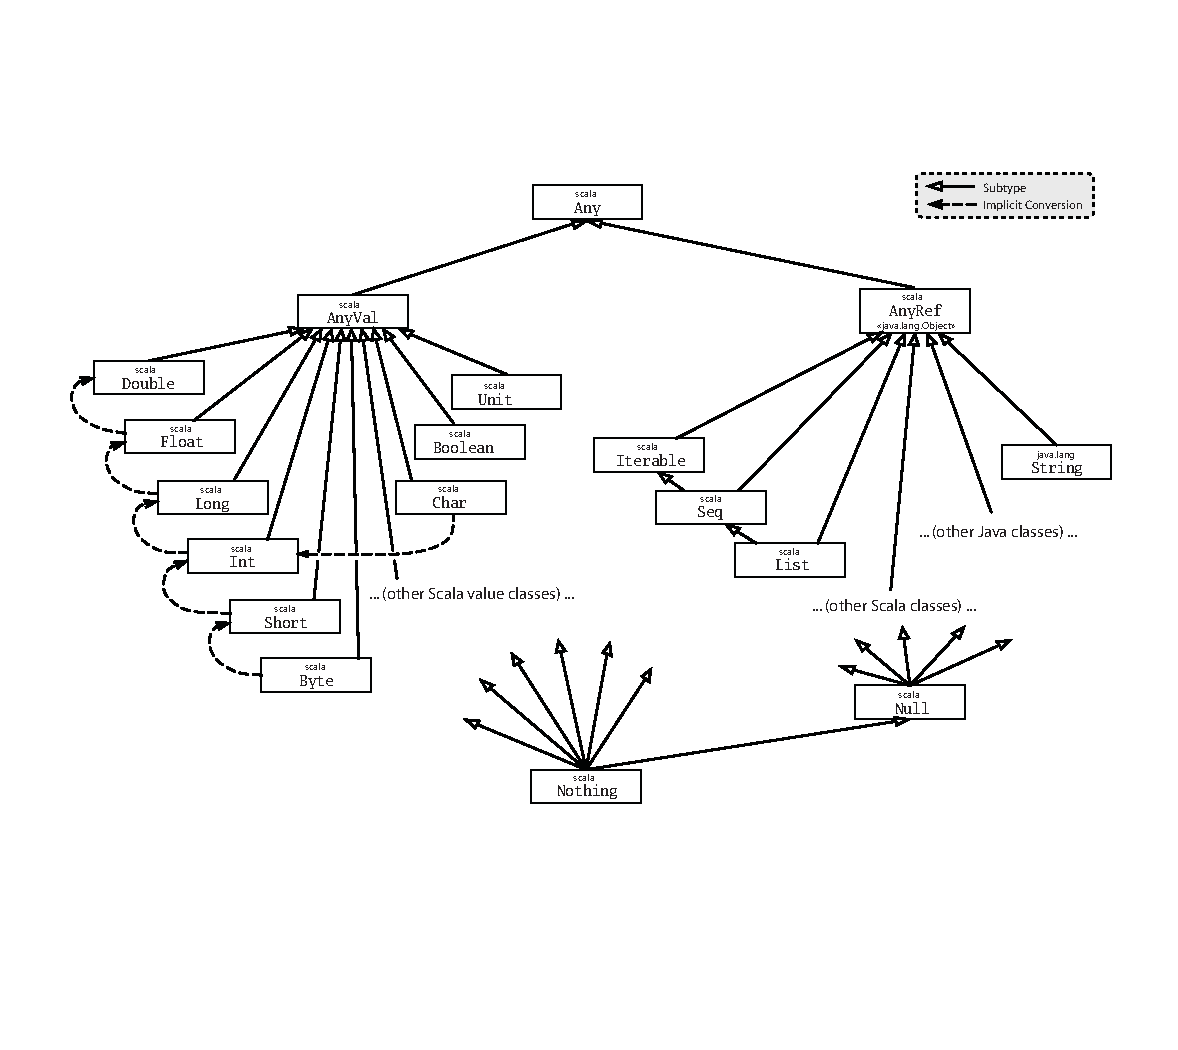
\includegraphics[width=1.07\textwidth,trim=12mm 0 0 0cm]{../img/hierarchy.pdf}

\Newline

{\small \renewcommand{\arraystretch}{1.2}
\begin{tabular}{l  l l l l l}
Numeric types
& \textbf{name} & \textbf{\# bits} & \textbf{range} & \textbf{Litteral} & \textbf{JVM} \\ \cline{2-6} %\hline 
\\[-1em]
&\texttt{Byte}   &  8  & $-2^7$ ... $2^7-1$  & \texttt{0.toByte} & \texttt{byte} \\
&\texttt{Short}  &  16 & $-2^{15}$ ... $2^{15}-1$ & \texttt{0.toShort}  & \texttt{short} \\
&\texttt{Char}   &  16 & $0$ ... $2^{16}-1$ & \texttt{'0'} & \texttt{char} \\
&\texttt{Int}    &  32 & $-2^{15}$ ... $2^{15}-1$ & \texttt{0} &\texttt{int} \\
&\texttt{Long}   &  64 & $-2^{15}$ ... $2^{15}-1$ & \texttt{0L} &\texttt{long} \\
&\texttt{Float}  &  32 & ± $3.4028235 \cdot 10^{38}$  & \texttt{0F} &\texttt{float} \\
&\texttt{Double} &  64 & ± $1.7976931348623157 \cdot 10^{308}$ & \texttt{0.0} &\texttt{double} \\
\end{tabular}
}

\Newline\head{The Scala Standard Collection Library}
{
\small\renewcommand{\arraystretch}{1.1}
\begin{multicols}{2}
\texttt{scala.collection.}
\begin{tabular}{l l l}
\texttt{immutable.} & \texttt{mutable.} & methods with good performance: \\
\hline
\texttt{Vector} & \texttt{ArrayBuffer} & \texttt{head tail apply +: :+}\\
\texttt{List} &  \texttt{ListBuffer} &  \texttt{head +:}  \\
\texttt{Set} & \texttt{Set} & \texttt{contains~~+~~-}\\
\texttt{Map} & \texttt{Map} & \texttt{apply~~+~~-} \\
\end{tabular}

\vspace{0.2em}

\texttt{String} and \texttt{Array} are implicitly converted to \texttt{Seq}\\ making sequence methods work as for other collections. Allocate Int array of size n: \texttt{ new Array[Int](n)}


\columnbreak

\newcommand{\NodeSkip}{0.5cm}
\begin{center}
\tikzstyle{collectiontype}=[rectangle, draw=black,  thick, anchor=north, text width=1.7cm, rectangle split, rectangle split parts = 1]
\begin{tikzpicture}[node distance = \NodeSkip]
\node (Traversable) [collectiontype]  {\texttt{\centerline{Traversable}}};
\node (Iterable) [collectiontype, below = of Traversable]  {\texttt{\centerline{Iterable}}};        
\node (Seq) [collectiontype, below left = \NodeSkip and 0.05cm of Iterable,text width=1.0cm,]  {\texttt{\centerline{Seq}}}; 
\node (Set) [collectiontype, right = of Seq, text width=1.0cm,]  {\texttt{\centerline{Set}}};               
\node (Map) [collectiontype, right = of Set, text width=1.0cm,]  {\texttt{\centerline{Map}}};        
\node (Vector) [collectiontype, below left = \NodeSkip and -0.3cm of Seq, text width=1.0cm,]  {\texttt{\centerline{Vector}}};     
\node (List) [collectiontype, below right = \NodeSkip and -0.2cm of Seq, text width=1.0cm,]  {\texttt{\centerline{List}}};              
      
\draw[umlarrow] (Iterable.north) -- (Traversable.south);        
\draw[umlarrow] (Seq.north) -- (Iterable.south west);        
\draw[umlarrow] (Set.north) -- (Iterable.south);        
\draw[umlarrow] (Map.north) -- (Iterable.south east);        
\draw[umlarrow] (Vector.north) -- (Seq.south west);        
\draw[umlarrow] (List.north) -- (Seq.south east);        
\end{tikzpicture}
\end{center}
\end{multicols}
}

{\small Concrete implementations of Set include HashSet, ListSet and BitSet. The subtype SortedSet is implemented by TreeSet.
Concrete implementations of Map include HashMap and ListMap. The subtype SortedMap is implemented by TreeMap.

}

\clearpage

\head{Methods in trait \texttt{Traversable}}\Newline

{\small\renewcommand{\arraystretch}{1.2}
\begin{tabular}{l p{3.4cm} p{6.6cm}}
\textbf{What} & \textbf{Usage} & \textbf{Explanation} f is a function, pf is a partial funct., p is a predicate.\\ \hline
Traverse: & \texttt{xs foreach f} & Executes f for every element of xs. Return type Unit.\\ \cline{1-3}

  Add: & \texttt{xs ++ ys} & A collection with xs followed by ys.\\\cline{1-3}
  
  Map: & \texttt{xs map f} & A collection formed by applying f to every element in xs.\\ \cline{2-3}
       & \texttt{xs flatMap f} & A collection obtained by applying f (which must return a collection) to all elements in xs and concatenating the results.\\ \cline{2-3}
       & \texttt{xs collect pf} & The collection obtained by applying the pf to every element in xs for which it is defined (undefined ignored).\\ \cline{1-3}

  Convert: & \texttt{toVector toList toSeq toBuffer toArray} & Converts a collection. Unchanged if the run-time type already matches the demanded type.\\ \cline{2-3}
   & \texttt{toSet} & Converts the collection to a set; duplicates removed.\\ \cline{2-3}
   & \texttt{toMap} & Converts a collection of key/value pairs to a map. \\ \cline{1-3}

  Copy: & \texttt{xs copyToBuffer buf } & Copies all elements of xs to buffer buf. Return type Unit.\\ \cline{2-3}
   & \texttt{xs copyToArray (arr, s, n)} & Copies at most n elements of the collection to array arr starting at index s (last two arguments are optional). Return type Unit.\\ \cline{1-3}

  Size info: & \texttt{xs.isEmpty} & Returns true if the collection xs is empty.\\ \cline{2-3}
   & \texttt{xs.nonEmpty} & Returns true if the collection xs has at least one element.\\ \cline{2-3}
   & \texttt{xs.size} & Returns an \texttt{Int} with the number of elements in xs.\\ \cline{1-3}
   

  Retrieval: & \texttt{xs.head xs.last} &  	The first/last element of xs (or some elem, if order undefined).\\ \cline{2-3}
      & \texttt{xs.headOption \newline xs.lastOption} & The first/last element of xs (or some element, if no order is defined) in an option value, or \texttt{None} if xs is empty.\\ \cline{2-3}
      & \texttt{xs find p} & An option with the first element satisfying p, or None.\\ \cline{1-3}


  Subparts: & \texttt{xs.tail xs.init} & The rest of the collection except xs.head or xs.last.\\ \cline{2-3}
      & \texttt{xs slice (from, to)} & The elements in from index \texttt{from} until (not including) \texttt{to}.\\ \cline{2-3}
      & \texttt{xs take n} & The first n elements (or some n elements, if order undefined).\\ \cline{2-3}
      & \texttt{xs drop n} & The rest of the collection except xs take n.\\ \cline{2-3}
      & \texttt{xs takeWhile p} & The longest prefix of elements all satisfying p.\\ \cline{2-3}
      & \texttt{xs dropWhile p} & Without the longest prefix of elements that all satisfy p.\\ \cline{2-3}
      & \texttt{xs filter p} & Those elements of xs that satisfy the predicate p. \\ \cline{2-3}
      & \texttt{xs filterNot p} & Those elements of xs that do not satisfy the predicate p.\\ \cline{2-3}
      & \texttt{xs splitAt n} &  	Split xs at n returning the pair (xs take n, xs drop n).\\ \cline{2-3}
      & \texttt{xs span p} & Split xs by p into the pair (xs takeWhile p, xs.dropWhile p).\\ \cline{2-3}
      & \texttt{xs partition p} & Split xs by p into the pair (xs filter p, xs.filterNot p)\\ \cline{2-3}
      & \texttt{xs groupBy f} & Partition xs into a map of collections according to f.\\ \cline{1-3}


  Conditions: & \texttt{xs forall p} & Returns true if p holds for all elements of xs.\\ \cline{2-3}
      & \texttt{xs exists p} & Returns true if p holds for some element of xs.\\ \cline{2-3}
      & \texttt{xs count p} & An \texttt{Int} with the number of elements in xs that satisfy p.\\ \cline{1-3}

  Folds: & \texttt{xs.foldLeft(z)(op) xs.foldRight(z)(op)} & Apply binary operation op between successive elements of xs, going left to right (or right to left) starting with z.\\ \cline{2-3}
      & \texttt{xs reduceLeft op \newline xs reduceRight op} & Similar to foldLeft/foldRight, but xs must be non-empty, starting with first element instead of z.\\ \cline{2-3}
      & \texttt{xs.sum xs.product xs.min xs.max} & Calculation of the sum/product/min/max of the elements of xs, which must be numeric.\\ \cline{1-3}
                              
   Make string: & \texttt{xs mkString (start, sep, end)} & A string with all elements of xs between separators sep enclosed in strings start and end; start, sep, end are all optional.\\ \cline{1-3}

   
\end{tabular}
}

\clearpage

\head{Methods in trait \texttt{Iterable}}\Newline

{\small\renewcommand{\arraystretch}{1.1}
\begin{tabular}{l p{3.4cm} p{6.8cm}}

\textbf{What} & \textbf{Usage} & \textbf{Explanation} \\ \hline

  Iterators: & \texttt{val it = xs.iterator} & An iterator \texttt{it} of type \texttt{Iterator} that yields each element one by one: \texttt{ while (it.hasNext) f(it.next)}\\   \cline{2-3}

   & \texttt{xs grouped size} & An iterator yielding fixed-sized chunks of this collection.\\\cline{2-3}
   & \texttt{xs sliding size} & An iterator yielding a sliding fixed-sized window of elements.\\\cline{1-3}

  Subparts: & \texttt{xs takeRight n \newline xs dropRight n} & Similar to \texttt{take} and \texttt{drop} in \texttt{Traversable} but takes/drops the last n elements (or any n elements if the order is undefined).\\   \cline{1-3}

  Zippers: & \texttt{xs zip ys} &  	An iterable of pairs of corresponding elements from xs and ys.\\   \cline{2-3}
   & \texttt{xs zipAll (ys, x, y)} & Similar to \texttt{zip}, but the shorter sequence is extended to match the longer one by appending elements x or y.\\\cline{2-3}
   & \texttt{xs.zipWithIndex} & An iterable of pairs of elements from xs with their indices.\\\cline{1-3}

  Compare: & \texttt{xs sameElements ys} & True if xs and ys contain the same elements in the same order.\\   \cline{1-3}

        
\end{tabular}
}  

\Newline
\head{Methods in trait \texttt{Seq}}\Newline

{\small\renewcommand{\arraystretch}{1.1}
\begin{tabular}{l p{3.75cm} p{6.6cm}}

%\textbf{What} & \textbf{Usage} & \textbf{Explanation} \texttt{f} is function, \texttt{pf} is partial funct., \texttt{p} is predicate.\\ \hline

  Indexing & \texttt{xs(i)  ~ xs apply i} & The element of xs at index i.\\   \cline{2-3}

   and size: & \texttt{xs.length} & Length of sequence. Same as \texttt{size} in \texttt{Traversable}.\\\cline{2-3}
   & \texttt{xs.indices} & Returns a \texttt{Range} extending from 0 to xs.length - 1.\\\cline{2-3}
   & \texttt{xs isDefinedAt i} & True if i is contained in xs.indices.\\\cline{2-3}
   & \texttt{xs lengthCompare n} & Returns -1 if xs is shorter than n, +1 if it is longer, else 0. \\\cline{1-3}

  
  Index & \texttt{xs indexOf x} & The index of the first element in xs equal to x.\\   \cline{2-3}
  search: & \texttt{xs lastIndexOf x} & The index of the last element in xs equal to x.\\\cline{2-3}
   & \texttt{xs indexOfSlice ys \newline xs lastIndexOfSlice ys} & The (last) index of xs such that successive elements starting from that index form the sequence ys.\\\cline{2-3}
   & \texttt{xs indexWhere p} & The index of the first element in xs that satisfies p.\\\cline{2-3}
   & \texttt{xs segmentLength (p, i)} & The length of the longest uninterrupted segment of elements in xs, starting with xs(i), that all satisfy the predicate p.\\\cline{2-3}
   & \texttt{xs prefixLength p} &  	Same as \texttt{ xs.segmentLength(p, 0)}\\\cline{1-3}


  Add: & {\texttt{x~+:~xs~~~~~xs~:+~x}}  & Prepend/Append x to xs. Colon on the collection side. \\   \cline{2-3}
   & \texttt{xs padTo (len, x)} & Append the value x to xs until length len is reached.\\\cline{1-3}
        

  Update: & \texttt{xs patch (i, ys, r)} &  A copy of xs with r elements of xs replaced by ys starting at i. \\   \cline{2-3}
   & \texttt{xs updated (i, x)} & A copy of xs with the element at index i replaced by x.\\\cline{2-3}
   & \texttt{xs(i) = x \newline xs.update(i, x)} & Only available for mutable sequences. Changes the element of xs at index i to x. Return type Unit.\\\cline{1-3}
        

  Sort: & \texttt{xs.sorted} & A new Seq[A] sorted using implicitly available ordering of A. \\   \cline{2-3}
   & \texttt{xs sortWith lt} &  	A new Seq[A] sorted using less than lt: (A, A) => Boolean.\\\cline{2-3}
   & \texttt{xs sortBy f} &  	A new Seq[A] sorted using implicitly available ordering of B after applying f: A => B to each element.\\ \cline{1-3}
        

  Reverse: & \texttt{xs.reverse} & A new sequence with the elements of xs in reverse order. \\   \cline{2-3}
   & \texttt{xs.reverseIterator} & An iterator yielding all the elements of xs in reverse order.\\\cline{2-3}
   & \texttt{xs reverseMap f} & Similar to map in Traversable, but in reverse order.\\\cline{1-3}
        

  Tests: & \texttt{xs startsWith ys} & True if xs starts with sequence ys. \\   \cline{2-3}
   & \texttt{xs endsWith ys} & True if xs ends with sequence ys.\\\cline{2-3}
   & \texttt{xs contains x} & True if xs has an element equal to x.\\\cline{2-3}
   & \texttt{xs containsSlice ys} & True if xs has a contiguous subsequence equal to ys\\\cline{2-3}
   & \texttt{(xs corresponds ys)(p)} & True if corresponding elements satisfy the binary predicate p.\\\cline{1-3}
   
  Subparts: & \texttt{xs intersect ys} & The intersection of xs and ys, preserving element order.\\\cline{2-3}
   & \texttt{xs diff ys} & The difference of xs and ys, preserving element order.\\\cline{2-3}
   & \texttt{xs union ys} & Same as \texttt{xs ++ ys} in Traversable.\\\cline{2-3}
   & \texttt{xs.distinct} & A subsequence of xs that contains no duplicated element.\\\cline{1-3}
                   
       
        
\end{tabular}
}  

%\Newline
\head{Methods in trait \texttt{Set}}\Newline

{\small\renewcommand{\arraystretch}{1.15}
\begin{tabular}{p{5cm}  p{6.6cm}}

%\textbf{Usage} & \textbf{Explanation} \\ \hline

\texttt{xs(x)~~~xs~apply~x} & True if x is a member of xs. Also: xs contains x\\   \cline{1-2}

\texttt{xs subsetOf ys} & True if ys is a subset of xs.\\\cline{1-2}

\texttt{xs~+~x~~~~~~~~~~xs - x} \newline \texttt{xs~+~(x,~y,~z)~~xs~-~(x,~y,~z)}& Returns a new set including/excluding elements. \newline Addition/subtraction can be applied to many arguments.\\   \cline{1-2}

\texttt{xs intersect ys} & A new set with elements in both xs and ys. Also: \texttt{\&} \\\cline{1-2}
\texttt{xs union ys} & A new set with elements in either xs or ys or both. Also: \texttt{|} \\\cline{1-2}
\texttt{xs diff ys} & A new set with elements in xs that are not in ys. Also: \texttt{\&\textasciitilde} \\\cline{1-2}
        
\end{tabular}
}  

\Newline
\head{Additional methods only in trait \texttt{mutable.Set}}\Newline
{\small\renewcommand{\arraystretch}{1.15}
\begin{tabular}{p{5cm}  p{6.6cm}}

\texttt{xs~+=~x~~~~~~~~~~xs~-=~x} \newline \texttt{xs~+=~(x,~y,~z)~~xs~-=~(x,~y,~z)}& Returns the same set with included/excluded elements. \newline Addition/subtraction can be applied to many arguments.\\   \cline{1-2}

\texttt{xs ++= ys} & Adds all elements in ys to set xs and returns xs itself. \\\cline{1-2}

\texttt{xs add x} & Adds element x to xs and returns true if x was in xs, else false. \\\cline{1-2}
\texttt{xs remove x} & Removes x from xs and returns true if x was in xs, else false. \\\cline{1-2}

\texttt{xs retain p} & Keeps only those elements in xs that satisfy predicate p.\\   \cline{1-2}
\texttt{xs.clear} &  	Removes all elements from xs. Return type Unit.\\   \cline{1-2}
\texttt{xs(x) = b ~~~ xs.update(x, b)} & If b is true, adds x to xs, else removes x. Return type Unit.\\   \cline{1-2}
\texttt{xs.clone} & Returns a new mutable set with the same elements as xs.\\   \cline{1-2}
        
\end{tabular}
}  

\Newline
\head{Methods in trait \texttt{Map}}\Newline

{\small\renewcommand{\arraystretch}{1.15}
\begin{tabular}{p{5.0cm}  p{6.6cm}}

\texttt{ms get k} & The value associated with key k an option, None if not found.\\   \cline{1-2}

\texttt{ms(k)~~~xs~apply~k} & The value associated with key k, or exception if not found.\\   \cline{1-2}

\texttt{ms getOrElse (k, d)} & The value associated with key k in map ms, or d if not found.\\   \cline{1-2}

\texttt{ms isDefinedAt k} & True if ms contains a mapping for key k. Also: ms.contains(k) \\   \cline{1-2}


\texttt{ms + (k -> v)  ~~ ms + ((k, v))} \newline \texttt{ms updated (k, v)} & The map containing all mappings of ms as well as the mapping k -> v from key k to value v. Also: ms + (k -> v, l -> w) \\   \cline{1-2}

\texttt{ms - k} & Excluding any mapping of key k. Also: ms - (k, l, m)\\   \cline{1-2}

\texttt{ms ++ ks ~~~~ ms {-}{-} ks} & The mappings of ms with the mappings of ks added/removed.\\   \cline{1-2}

\texttt{ms.keys  ~~~~~ ms.values} & An iterable containing each key/value in ms.\\   \cline{1-2}
        
\end{tabular}
}  


\Newline
\head{Additional methods only in trait \texttt{mutable.Map}}\Newline

{\small\renewcommand{\arraystretch}{1.15}
\begin{tabular}{p{5.0cm}  p{6.8cm}}

\texttt{ms(k) = v ~~ ms.update(k, v)} & Adds mapping k to v, overwriting any previous mapping of k.\\   \cline{1-2}

\texttt{ms += (k -> v) ~~~~ ms -= k} & Adds/Removes mappings. Also vid several arguments.\\   \cline{1-2}

\texttt{ms put (k, v) ~~~ ms remove k}& Adds/removes mapping; returns previous value of k as an option.\\   \cline{1-2}

\texttt{ms retain p} & Keeps only mappings that have a key satisfying predicate p.\\   \cline{1-2}

\texttt{ms.clear} & Removes all mappings from ms.\\   \cline{1-2}

\texttt{ms transform f} & Transforms all associated values in map ms with function f.\\   \cline{1-2}

\code|ms.clone| & Returns a new mutable map with the same mappings as ms.\\   \cline{1-2}
        
\end{tabular}
}  
\vspace{0.5em}

\textbf{\color{\LangColor}{Factory methods examples}:}
{\small \texttt{ Vector(0, 0, 0) } same as \texttt{ Vector.fill(3)(0)} 
\texttt{ collection.mutable.Set.empty[Int]; Map("se" -> "Sweden", "dk" -> "Denmark")
\newline Array.ofDim[Int](3,2)} gives \texttt{Array(Array(0, 0), Array(0, 0), Array(0, 0))} same as \texttt{Array.fill(3,2)(0)}; 
\texttt{ Vector.iterate(1.2, 3)(\_ + 0.5)} gives \texttt{Vector(1.2, 1.7, 2.2)}; 
\newline \texttt{ Vector.tabulate(3)("s" + \_) } gives \code{ Vector("s0", "s1", "s2")}
}



\Newline\head{String methods}\Newline


{\small\renewcommand{\arraystretch}{1.15}

Some methods below are from java.lang.String and some methods are implicitly added from StringOps, etc.\\ Strings are implictly treated as Seq[Char] so all Seq methods also works.

\vspace{0.5em}

\begin{tabular}{l l}
\code|s.capitalize| & Returns this string with first character converted to upper case. \\
\code|s(i)  s apply i   s.charAt(i)| & Returns the character at index i. \\
\code|s.compareTo(t)| & Returns x where x < 0 if s < t, x > 0 if s > t, x is 0 if s == t\\
\code|s.compareToIgnoreCase(t)| & Similar to compateTo but not sensitive to case.\\
\code|s.endsWith(t)| & True if string s ends with string t. \\
\code|s.replaceAllLiterally(s1, s2)| & Replace all occurances of s1 with s2 in s. \\
\code|s.split(c)| & Returns an array of strings split at every occurance of charachter c. \\
\code|s.startsWith(t)| & True if string s begins with string t. \\
\code|s.stripMargin| & Strips leading white space followed by | from each line in string.\\
\code|s.substring(i)| & Returns a substring of s with all charcters from index i.\\
\code|s.substring(i, j)| & Returns a substring of s from index i to index j-1.\\
\code|s.toInt  s.toDouble  s.toFloat| & Parses s as an Int or Double etc. May throw an exception.\\
\code|42.toString   42.0.toString| & Converts a number to a String.\\
\code|s.toLowerCase| & Converts all characters to lower case.\\
\code|s.toUpperCase| & Converts all characters to upper case. \\
\code|s.trim| & Removes leading and trailing white space.\\
\end{tabular}
} 



\Newline\head{scala.collection.JavaConverters}\Newline

{\small
Enable \code{.asJava} and \code{.asScala} conversions: \code{ import collection.JavaConverters._ } 
\vspace{0.5em}

\begin{tabular}{r c l}
\texttt{xs.asJava} on a \textbf{Scala} collection of type: & & \texttt{xs.asScala} on a \textbf{Java} collection of type: \\ 
\texttt{Iterator} &               $\longleftrightarrow$ & \texttt{java.util.Iterator} \\
\texttt{Iterable} &               $\longleftrightarrow$ & \texttt{java.lang.Iterable} \\
\texttt{Iterable} &               $\leftarrow$ & \texttt{java.util.Collection} \\
\texttt{mutable.Buffer} &         $\longleftrightarrow$  & \texttt{java.util.List} \\
\texttt{mutable.Set} &            $\longleftrightarrow$  & \texttt{java.util.Set} \\
\texttt{mutable.Map} &            $\longleftrightarrow$  & \texttt{java.util.Map} \\
\texttt{mutable.ConcurrentMap} &  $\longleftrightarrow$  & \texttt{java.util.concurrent.ConcurrentMap} \\\end{tabular}
}


\Newline\head{Special characters and strings}\Newline

{\small\renewcommand{\arraystretch}{1.15}
\begin{tabular}{p{0.6cm} l | r l}
\textbf{Escape\newline char} &  & \textbf{String} & \\ 
\code|\n| & line break & \code|"hello\nworld"| & string including escape char for line break\\
\code|\t| & horisontal tab & \code|"""a "raw" string"""| & can include quotes and span multiple lines\\
\code|\"| & double quote '' & \code|s"x is $x"| & the s interpolator inserts values of existing names\\
\code|\'| & single quote ' &  \code|s"x+1 is ${x+1}"|& the s interpolator evaluates expressions within  \code|${}|\\
\code|\\| & backslash \textbackslash &  & \\
\end{tabular}
} 


\Newline\head{Reserved words}\Newline

{\small The 40 words and 10 symbols below have special meaning and cannot be used as identifiers in Scala.}
 
\begin{Code}[morekeywords={macro,\_},otherkeywords={>,<-,\%,<,>:,@,:,=,\#}]
abstract case catch class def do else extends false final 
finally for forSome if implicit import lazy macro match new 
null object override package private protected return sealed 
super this throw trait try true type val var while with yield 
_   :   =   =>   <-   <:   <%   >:   #   @ 
\end{Code}




\clearpage
\setcounter{page}{1}
\renewcommand{\LangColor}{blue}
\LangMarker{Java}{3.5cm}

\LangTitle{Java snabbreferens}

{\small Tecknet ~\Or~ står för ''eller''. Vanliga parenteser \RepL \RepR ~används för att gruppera alternativ. Med \OptL \OptR ~markeras sådant som inte alltid finns med. Med \jcode{stmt} avses en sats, \jcode{x}, \jcode{i}, \jcode{s}, \jcode{ch} är variabler, \jcode{expr} är ett uttryck, \jcode{cond} är ett logiskt uttryck.}

\Newline
\head{Satser}

\begin{etab}
Block   & \jcode|{stmt1; stmt2; ...}| &  fungerar ''utifrån'' som \textbf{en} sats \secend

Tilldelningssats & \jcode|x = expr;|                 &  variabeln och uttrycket av kompatibel typ \secend

Förkortade       & \jcode|x += expr; |                &  x = x + expr; även --=, *=, /= \\
                 & \jcode|x++;  |                     &  x = x + 1; även x\hspace{0.5mm}-- -- \secend

if-sats          & \jcode|if (cond) {stmt; ...}|      &  utförs om cond är true \\
                 & \OptL \jcode|else { stmt; ...}| \OptR&  utförs om false \secend

switch-sats      & \jcode|switch (expr) {|         &  expr är ett heltalsuttryck \\ 
                 & \jcode|    case A: stmt1; break;|  &  utförs om expr $=$ A (A konstant) \\
                 & \jcode|    ...|                 & \\
                 & \jcode|    default: stmtN; break;| &  utförs om inget case passar\\
                 & \jcode|}|                   & \secend

for-sats         & \jcode|for (int i = start; i < stop; i++) {| & \\
                 & \jcode|    stmt;|  & satserna utförs för i = start, start+1, \ldots, stop$-1$ \\
                 & \jcode|    ...;|         &  (ingen gång om start >= stop) \\
                 & \jcode|}|                &  i++ kan ersättas med i = i + step \secend

while-sats       & \jcode|while (cond) {|          & \\
                 & \jcode|    stmt; ...|           &  utförs så länge cond är true \\
                 & \jcode|}|                       & \secend

do-while-sats    & \jcode|do {|                     & \\
                 & \jcode|    stmt; ...|         &  utförs minst en gång, \\
                 & \jcode|} while (cond);|          &  så länge cond är true \secend

return-sats      & \jcode|return expr;|        &  returnerar funktionsresultat
\end{etab}

\head{Uttryck}
\begin{etab}
Aritmetiskt uttryck & (x + 2) * i / 3          &  skrivs som i matematiken, för heltal är / \\
                  &                            &  heltalsdivision, \% ''rest'' \secend

Objektuttryck     & \mc{new Classname(\ldots) | ref-var | null | function-call | this | super} \secend

Logiskt uttryck   & \mc{! log-expr | log-expr \&\& log-expr | log-expr || log-expr | function-call | relation | log-var | true | false} \subsecend

Relation          & \mc{ expr ( < | <= | == | >= | > | != ) expr (för objektuttryck bara == och !=, också expr instanceof Classname)} \subsecend

Funktionsanrop    & obj-expr.method(\ldots)    &  anropa ''vanlig metod'' (utför operation) \\
                  & Classname.method(\ldots)   &  anropa statisk metod \secend

Vektor (array)    & new int[size]              &  skapar int-vektor med size element \\
                  & vname[i]                   &  elementet med index i, 0..length$-1$\\
                  & vname.length               &  antalet element \secend

Typkonvertering   & (newtype) expr             &  konverterar expr till typen newtype \\
                  & (int) real-expr            &  -- avkortar genom att stryka decimaler \\
                  & (Square) aShape            &  -- ger ClassCastException om aShape inte \\
                  &                            &  är ett Square-objekt
\end{etab}

\clearpage 
\head{Deklarationer}
\begin{etab}
Allmänt           & \mc{[<protection>] [static] [final] <type> name1, name2, \ldots;} \secend

<type>            & \mc{byte | short | int | long | float | double | boolean | char | Classname} \secend

<protection>      & public | private | protected &  för attribut och metoder i klasser \\
                  &                             &  (paketskydd om inget anges) \secend

Startvärde        & int x = 5;                  &  startvärde bör alltid anges \secend

Konstant          & final int N = 20;           &  konstantnamn med stora bokstäver \secend

Vektor            & <type>[\hspace{0.4mm}] vname = new <type>[10]; &  deklarerar och skapar vektor
\end{etab}


\head{Klasser}
\begin{etab}
Deklaration       & [public][abstract] class Classname & \\
                  & \mc{\ind [extends Classname1] [implements Interface1, Interface2, \ldots] $\{$} \\
                  & \ind <deklaration av attribut> & \\
                  & \ind <deklaration av konstruktorer> & \\
                  & \ind <deklaration av metoder> & \\
                  & $\}$                          & \secend

Attribut          & \mc{Som vanliga deklarationer. Attribut får implicita startvärden, 0, 0.0, false, null.} \secend

Konstruktor       & <prot> Classname(param, \ldots) $\{$ &  Parametrarna är de parametrar som ges vid \\
                  & \ind stmt; \ldots              &  new Classname(\ldots). Satserna ska ge \\ 
                  & $\}$                           &  attributen startvärden \secend

Metod             & <prot> <type> name(param, \ldots) $\{$ &  om typen inte är void måste en return-\\
                  & \ind stmt; \ldots              &  sats exekveras i metoden \\
                  & $\}$                           & \secend
                  
Huvudprogram      & \mc{public static void main(String[\hspace{0.5mm}] args) $\{$ \ldots $\}$} \secend

Abstrakt metod    & \mc{Som vanlig metod, men abstract före typnamnet och $\{\ldots\}$ ersätts med semikolon. Metoden måste implementeras i subklasserna.}
\end{etab}

\head{Standardklasser, java.lang, behöver inte importeras}
\begin{etab}
Object            & \mc{Superklass till alla klasser.} \subsecend
                  & boolean equals(Object other);   &  ger true om objektet är lika med other \\
                  & int hashCode();                 &  ger objektets hashkod \\
                  & String toString();              &  ger en läsbar representation av objektet \secend
                  
Math              & \mc{Statiska konstanter Math.PI och Math.E. Metoderna är statiska (anropas med t~ex Math.round(x)):} \subsecend
                  & long round(double x);           &  avrundning, även float $\rightarrow$ int \\
                  & int abs(int x);                 &  $|x|$, även double, \ldots \\
                  & double hypot(double x, double y); &  $\sqrt{x^2+y^2}$ \\
                  & double sin(double x);           &  $\sin x$, liknande: cos, tan, asin, acos, atan \\
                  & double exp(double x);           &  $e^x$ \\
                  & double pow(double x, double y); &  $x^y$ \\
                  & double log(double x);           &  $\ln x$ \\
                  & double sqrt(double x);          &  $\sqrt{x}$ \\
                  & double toRadians(double deg);   &  $\mathit{deg} \cdot \pi / 180$ \secend

System            & void System.out.print(String s); &  skriv ut strängen s \\
                  & void System.out.println(String s); &  som print men avsluta med ny rad \\
                  & void System.exit(int status);   &  avsluta exekveringen, status != 0 om fel \\
                  & \mc{Parametern till print och println kan vara av godtycklig typ: int, double, \ldots} \secend
\end{etab}
\clearpage
\begin{etab}
Typklasser        & \mc{Till varje datatyp finns en typklass: char $\rightarrow$ Character, int $\rightarrow$ Integer, double $\rightarrow$ Double, \ldots\ Statiska konstanter MIN\_VALUE och MAX\_VALUE ger minsta respektive största värde. Exempel med klassen Integer:} \subsecend
                  & Integer(int value);             &  skapar ett objekt som innehåller value \\
                  & int intValue();                 &  tar reda på värdet \secend

String            & \mc{Teckensträngar där tecknen inte kan ändras. ''asdf'' är ett String-objekt. s1 + s2 för att konkatenera två strängar. StringIndexOutOfBoundsException om någon position är fel.} \subsecend
                  & int length();                   &  antalet tecken \\
                  & char charAt(int i);             &  tecknet på plats i, 0..length()$-1$ \\
                  & boolean equals(String s);       &  jämför innehållet (s1 == s2 fungerar inte) \\
                  & int compareTo(String s);        &  < 0 om mindre, = 0 om lika, > 0 om större \\
                  & int indexOf(char ch);           &  index för ch, $-1$ om inte finns \\
                  & int indexOf(char ch, int from); &  som indexOf men börjar leta på plats from \\
                  & String substring(int first, int last); &  kopia av tecknen first..last$-1$ \\
                  & String[\hspace{0.5mm}] split(String delim); &  ger vektor med ''ord'' (ord är följder av \\
                  &                                 &  tecken åtskilda med tecknen i delim) \secend

                  & \mc{Konvertering mellan standardtyp och String (exempel med int, liknande för andra typer):} \subsecend
                  & String.valueOf(int x);          &  x = 1234 $\rightarrow$ ''1234'' \\ 
                  & Integer.parseInt(String s);     &  s = ''1234'' $\rightarrow$ 1234, NumberFormat- \\
                  &                                 &  Exception om s innehåller felaktiga tecken \secend

StringBuilder     & \mc{Modifierbara teckensträngar. length och charAt som String, plus:} \subsecend
                  & StringBuilder(String s);        &  StringBuilder med samma innehåll som s \\
                  & void setCharAt(int i, char ch); &  ändrar tecknet på plats i till ch \\
                  & StringBuilder append(String s); &  lägger till s, även andra typer: int, char, \ldots \\
                  & StringBuilder insert(int i, String s); &  lägger in s med början på plats i \\
                  & StringBuilder deleteCharAt(int i); &  tar bort tecknet på plats i \\ 
                  & String toString();              &  skapar kopia som String-objekt
\end{etab}

\head{Standardklasser, import java.util.Classname}
\begin{etab}
List              & \mc{List<E> är ett gränssnitt som beskriver listor med objekt av parameterklassen E. Man kan lägga in värden av standardtyperna genom att kapsla in dem, till exempel int i Integer-objekt. Gränssnittet implementeras av klasserna ArrayList<E> och LinkedList<E>, som har samma operationer. Man ska inte använda operationerna som har en position som parameter på en LinkedList (i stället en iterator). IndexOutOfBoundsException om någon position är fel.} \subsecend
                  & \mc{För att operationerna contains, indexOf och remove(Object) ska fungera måste klassen E överskugga funktionen equals(Object). Integer och de andra typklasserna gör det.} \subsecend
ArrayList         & ArrayList<E>();                 &  skapar tom lista \\ 
LinkedList        & LinkedList<E>();                &  skapar tom lista \\ 
                  & int size();                     &  antalet element \\
                  & boolean isEmpty();              &  ger true om listan är tom \\
                  & E get(int i);                   &  tar reda på elementet på plats i \\
                  & int indexOf(Object obj);        &  index för obj, $-1$ om inte finns \\
                  & boolean contains(Object obj);   &  ger true om obj finns i listan \\

                  & void add(E obj);                &  lägger in obj sist, efter existerande element \\
                  & void add(int i, E obj);         &  lägger in obj på plats i (efterföljande \\
                  &                                 &  element flyttas) \\
                  & \ldots\ forts nästa sida        & 
\end{etab}
\secend
\begin{etab}
                  & E set(int i, E obj);            &  ersätter elementet på plats i med obj \\
                  & E remove(int i);                &  tar bort elementet på plats i (efter- \\
                  &                                 &  följande element flyttas) \\
                  & boolean remove(Object obj);     &  tar bort objektet obj, om det finns \\
                  & void clear();                   &  tar bort alla element i listan \secend

Random            & Random();                       &  skapar ''slumpmässig'' slumptalsgenerator \\
                  & Random(long seed);              &  -- med bestämt slumptalsfrö \\
                  & int nextInt(int n);             &  heltal i intervallet [0, n) \\
                  & double nextDouble();            &  double-tal i intervallet [0.0, 1.0) \secend

Scanner           & Scanner(File f);                &  läser från filen f, ofta System.in \\
                  & Scanner(String s);              &  läser från strängen s \\
                  & String next();                  &  läser nästa sträng fram till whitespace \\
                  & boolean hasNext();              &  ger true om det finns mer att läsa \\
                  & int nextInt();                  &  nästa heltal; också nextDouble(), \ldots \\
                  & boolean hasNextInt();           &  också hasNextDouble(), \ldots \\
                  & String nextLine();              &  läser resten av raden
\end{etab}



\head{Filer, import java.io.File/FileNotFoundException/PrintWriter}
\begin{etab}
Läsa från fil     & \mc{Skapa en Scanner med new Scanner(new File(filename)). Ger File\-NotFoundException om filen inte finns. Sedan läser man ''som vanligt'' från scannern (nextInt och liknande).} \subsecend
                  
Skriva till fil   & \mc{Skapa en PrintWriter med new PrintWriter(new File(filename)). Ger FileNotFoundException om filen inte kan skapas. Sedan skriver man ''som vanligt'' på PrintWriter-objektet (println och liknande).}\subsecend

Fånga undantag    & \mc{Så här gör man för att fånga FileNotFoundException:\\[1mm]
\ind Scanner scan = null;\\
\ind try $\{$\\
\ind \ind scan = new Scanner(new File("indata.txt"));\\
\ind $\}$ catch (FileNotFoundException e) $\{$\\
\ind \ind \ldots\ ta hand om felet\\
\ind $\}$}
\end{etab}


\head{Specialtecken}
\begin{etab}
                  & \mc{Några tecken måste skrivas på ett speciellt sätt när de används i teckenkonstanter:}\subsecend

& \textbackslash{}n & ny rad, radframmatningstecken\\
& \textbackslash{}t & ny kolumn, tabulatortecken (eng. tab)\\
& \textbackslash{}\textbackslash{} & bakåtsnedstreck: \textbackslash{} (eng. {\em backslash})\\
& \textbackslash{}'' & citationstecken: ''\\
& \textbackslash{}' & apostrof: '\\

\end{etab}

\head{Reserverade ord}\Newline

{\small Nedan 50 ord kan ej användas som identifierare i Java. Orden \jcode{goto} och \jcode{const} är reserverade men används ej.}
 
\begin{Code}[language=Java,morekeywords={assert, enum, strictfp}]
abstract assert boolean break byte case catch char class const 
continue default do double else enum extends final finally float for 
goto if implements import instanceof int interface long native new 
package private protected public return short static strictfp super 
switch synchronized this throw throws transient try void volatile while
\end{Code}

\end{document}